%--------------------------------------------------
%	Chapter 5. GNN Pattern Recognition Algorithm
%--------------------------------------------------

\chapter{Graph Neural Network Pattern Recognition Algorithm}\label{chapter-5}

Once compatible hit-pairs from a particle collision event have been established, they can be used to build a graph network. This chapter presents a novel pattern recognition algorithm to prune outlier connections in such a network in order to reconstruct tracks, by utilising GNN architectures. The application of the GNN is focused on the Pixel detector, with the aim that the approach will serve as a sophisticated track seeding technique for Pixel hits and form preliminary track candidates. Such an approach could be efficient for saving vast computational resources if the GNN does not produce large proportions of fake tracks. The ultimate aim is to develop a realistic algorithm for fast track reconstruction that can be deployed in future high-luminosity phases of particle detector experiments. This research was presented at the 2022 Connecting the Dots (CTD) conference at the University of Princeton USA, as well as the dedicated GNN Google DeepMind seminar, held at UCL in 2023. At the time of writing this work was under review for publication in the Springer Journal: Computing for Software and Big Science \cite{Lad_2023_gnn}. Sections \ref{gnn-algorithm-overview} to \ref{gnn-track-extration} present a breakdown of the GNN algorithm and Section \ref{gnn-application-toy-model} illustrates an application on a simple toy model.


\section{Algorithm Overview}
\label{gnn-algorithm-overview}
The GNN based pattern recognition algorithm is considered an iterative mixture reduction task, which allows the deactivation of incompatible connections (GNN edges termed as outliers). This enables the improvement of track parameter estimates and iterative extraction of track candidates. 

Individual hits or clusters of hits are modelled as graph nodes and track segments are modelled as graph edges. Once the graph network is constructed, each edge is modelled as a Gaussian state in order to approximate the local track state probability density. Therefore, each node is initialised with a Gaussian mixture of track states, local to its neighbourhood of connections.

After initialisation, the network evolves iteratively, where an iteration is made up of three main stages illustrated in Figure \ref{fig:flowchart}. The first stage comprises of Gaussian Mixture Reduction (GMR). This involves a traditional ML approach, whereby compatible Gaussian states are grouped together using clustering techniques and outlier states can be identified. Following this, an Information Aggregation stage is executed, which leverages message passing between adjacent nodes in a given neighbourhood. The compatibility of neighbouring states can be assessed via extrapolation, in order to improve local track parameters using neighbourhood information. The third stage involves updating the network state at each node, as specific connections are deactivated as the network evolves. A graph splitting algorithm is also applied directly after the first two stages, in order to identify good track candidates, and if discovered they are extracted. 

Unlike traditional methodologies whereby Multi-Layered Perceptrons (MLPs) are employed for deep learning strategies, the proposed GNN leverages simplified KFs embedded in the network and are used for two main purposes. Firstly, the KF is used as a mechanism for information propagation during the second stage, in order to iteratively improve the precision of track parameters. The KF is also used within the extraction of track candidates to ensure compatibility with the particle motion model. This allows the model to efficiently exploit a prior knowledge about charged particle dynamics as the network evolves.

The excitation and inhibition rules of individual edge connections are designed to facilitate the “simple-to-complex” approach for “hits-to-tracks” association, such that the network starts with low hit density regions of an event and gradually progresses towards more complex areas. As the network evolves, the uncertainty in local track orientation decreases until there are no more track candidates that fulfil the criteria for a good track. This is the end state of the network where isolated nodes, track fragments and unresolved ambiguities will remain.

\begin{figure}[htbp]
    \centering
    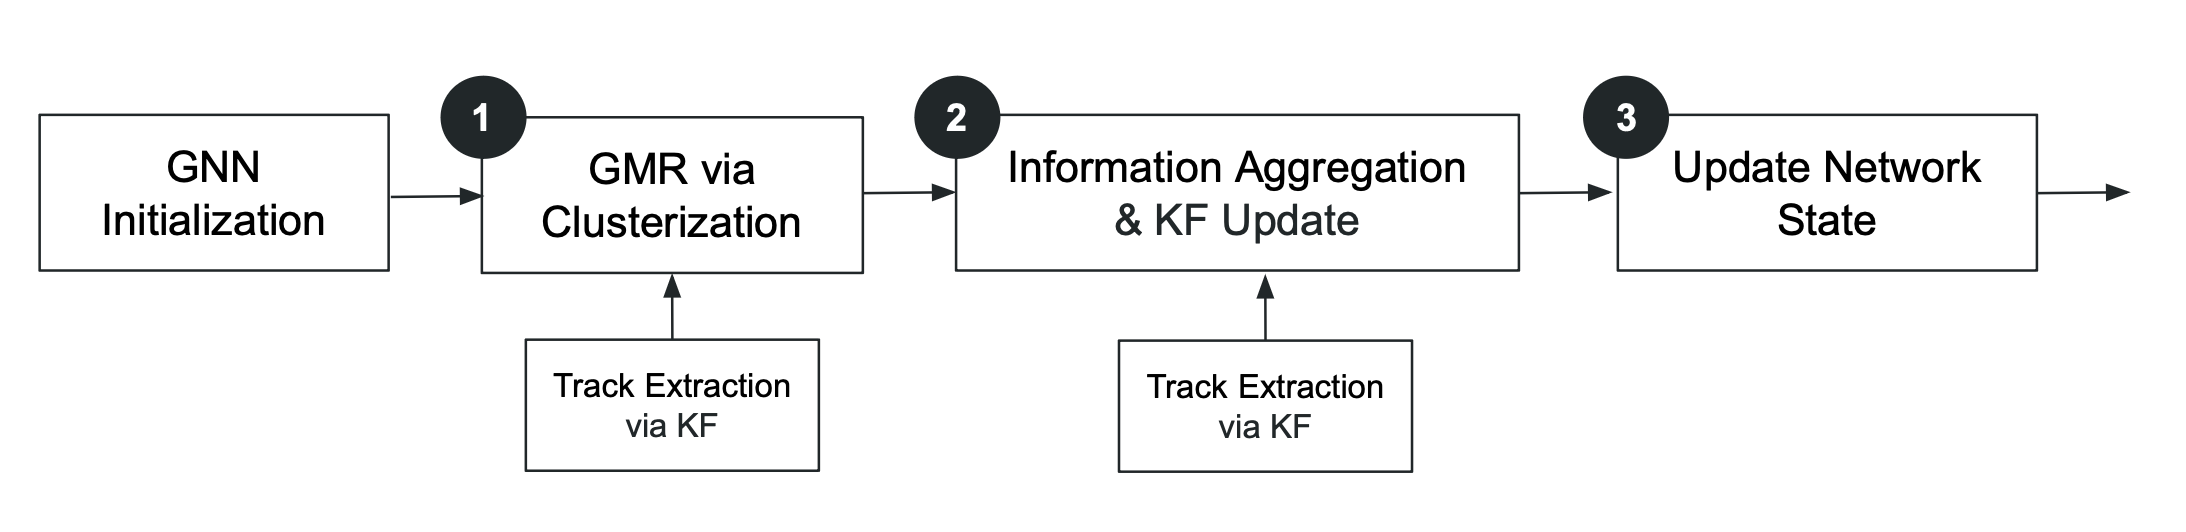
\includegraphics[width=0.98\textwidth]{images/5-gnn-algorithm/gnn-workflow.png}
    \caption{Flow chart illustrating all stages making up an iteration of the GNN-based algorithm. After each stage, a Kalman filter (KF) is applied in order to iteratively extract candidates. After stage three, a further Gaussian Mixture Reduction (GMR) stage would be applied repeating the iterations.}
    \label{fig:flowchart}%
\end{figure}



\section{Graph Network Initialization}
\label{gnn-network-initialization}

The graph network is constructed using the Python library \texttt{NetworkX} \cite{SciPyProceedings_11}. Hits from a particle event are represented as nodes and predicted hit-pairs as edge connections. See chapter \ref{chapter-4} for further details on the hit-pair predictor used to form edge connections. Following this, a common computer vision technique, known as Connected Component Analysis (CCA), is applied using a built-in function\cite{networkx}. CCA detects connected regions in data structures and allows the network to be split into smaller, more manageable graphs referred to as \textit{subgraphs}. 

Each pairwise connection between node $i$ and neighbour node $j$ forms a Gaussian state, $X_{ij}$, representing the local track parameter estimate. Each edge has an associated prior probability $p_{ij}$ and edge weight $w_{ij}$. The prior probability of node $i$ and neighbour node $j$ belonging to the same track is determined, assuming a track can produce at most one hit per layer of the detector. $w_{ij}$ is a mixture weight for the compatibility of the Gaussian state transmitted from node $i$ to neighbour node $j$, and represents the strength of the connection. $w_{ij}$ are initialised as uniform weights and are dependent on the number of neighbours local to a node. $w_{ij}$ and $p_{ij}$ are updated based on how the network evolves. $w_{ij}$ are not to be confused with the traditional weights associated to features within neural networks.

For a given node $i$ and neighbour nodes $j$, a Gaussian mixture $g_i(X)$ is formed from weighted components, $\phi_{ij}$, which describe the local neighbourhood and is given by Eq \eqref{eqn:gaussian-mixture},

\begin{equation}
g_i(X) = \sum_{j} w_{ij}\phi_{ij}(X, X_{ij}, C_{ij})
\label{eqn:gaussian-mixture}
\end{equation}

where $C_{ij}$ are the track state covariances. All edges act as bidirectional conduits, such that message passing can occur in both directions. All edges are initialised as \textit{active}, allowing the propagation of state information between its node-pair, whereas \textit{deactive} edges are defined to not allow state information to be propagated. 

%Figure \ref{fig:network-initial} illustrates a node and its neighbourhood.

% \begin{figure}[htbp]%
%     \centering
%     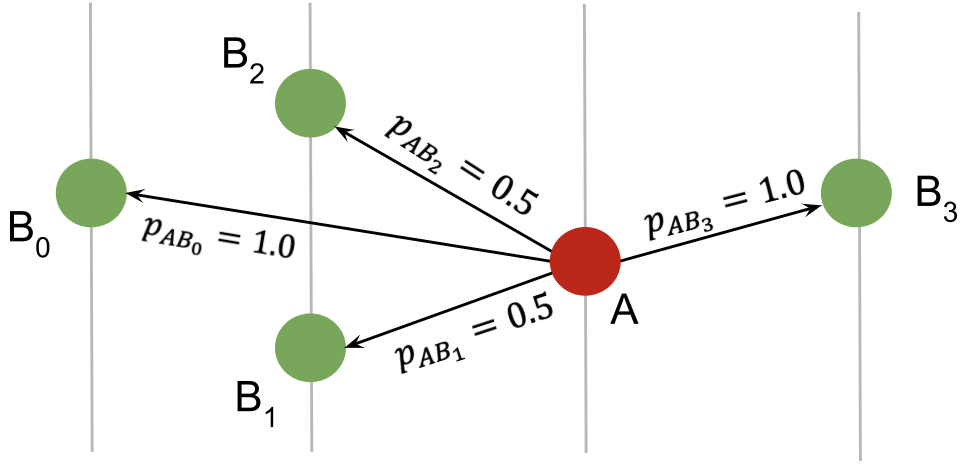
\includegraphics[width=8.8cm]{images/5-gnn-algorithm/network-initialisation.png}%
%     \caption{Prior probabilities associated to network edges of node A's local neighbourhood. Neighbours $B_j$ are located on separate detector layers shown by vertical lines. The unidirectional edges indicate the direction of propagation of state information and priors. These entities will differ from nodes $B_j$ distributing messages to their corresponding neighbourhoods.}%
%     \label{fig:network-initial}%
%\end{figure}




\section{Gaussian Mixture Reduction}
\label{section-GMR}
For nodes with a high multiplicity of edge connections, the number of track states can quickly rise. To make inferences within a reasonable amount of processing time, GMR is used to prevent the number of components from exploding. One computationally efficient algorithm for GMR is clustering. A high order Gaussian mixture can be approximated by one with lower order, using the traditional k-means clustering \cite{kmeans}. At each node, similar track states are grouped together forming a reduced mixture and their corresponding edges remain active, as illustrated in Figure \ref{fig:GMR-example}. Outlier states are simultaneously identified and their edges are deactivated. For a given node $i$, if clustering was successful the corresponding merged state estimate $X^{M}$ and merged state covariance $C^{M}$ is formed from the clustered states using the inverse-variance weighting \cite{inverse-variance-weighting} given by Eq \eqref{eqn:inverse-variance-weighting}, where $G_{ij}$ = $C_{ij}^{-1}$.

\begin{equation}
    X^{M} = C^{M} \sum_{j} G_{ij} X_{ij},  \quad  C^{M} = \left( \sum_{j} G_{ij} \right) ^{-1}
    \label{eqn:inverse-variance-weighting}
\end{equation}


\begin{figure}[htbp!] 
    \centering
    \subfloat[]{%
        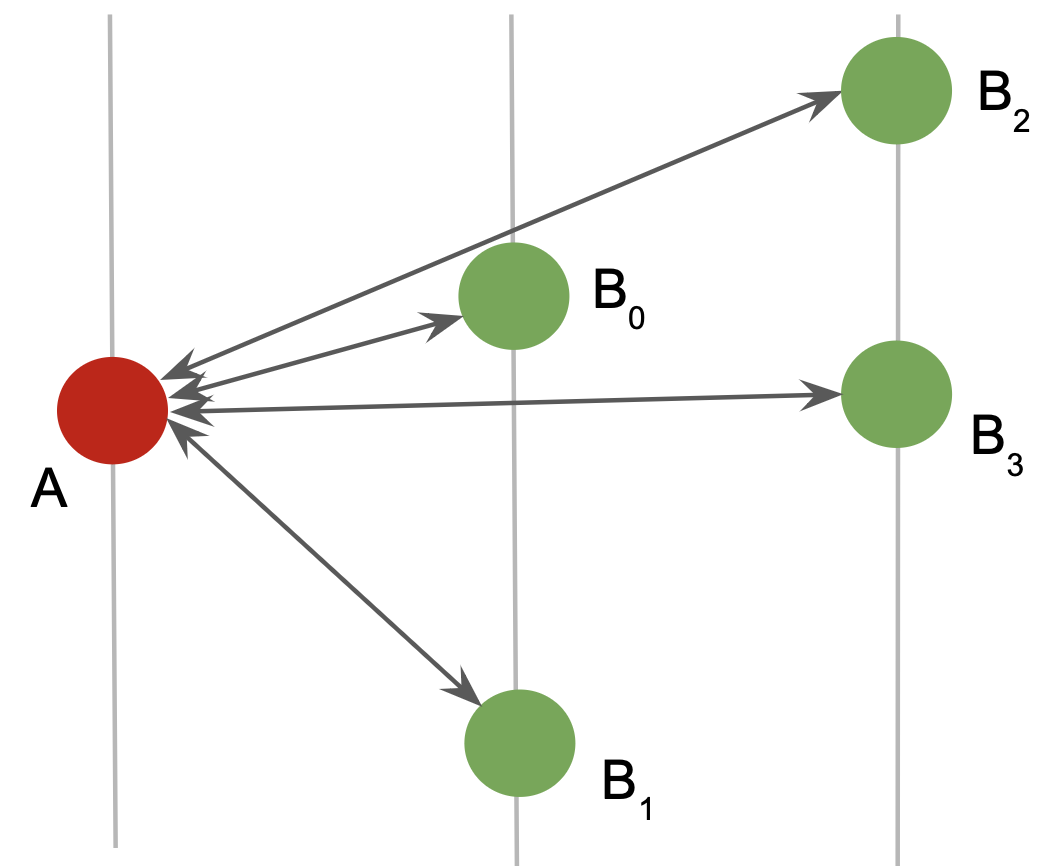
\includegraphics[width=0.42\linewidth]{images/5-gnn-algorithm/GMR-1.png}%
        \label{fig:GMR-1}%
        }%
    \hfill%
    \subfloat[]{%
        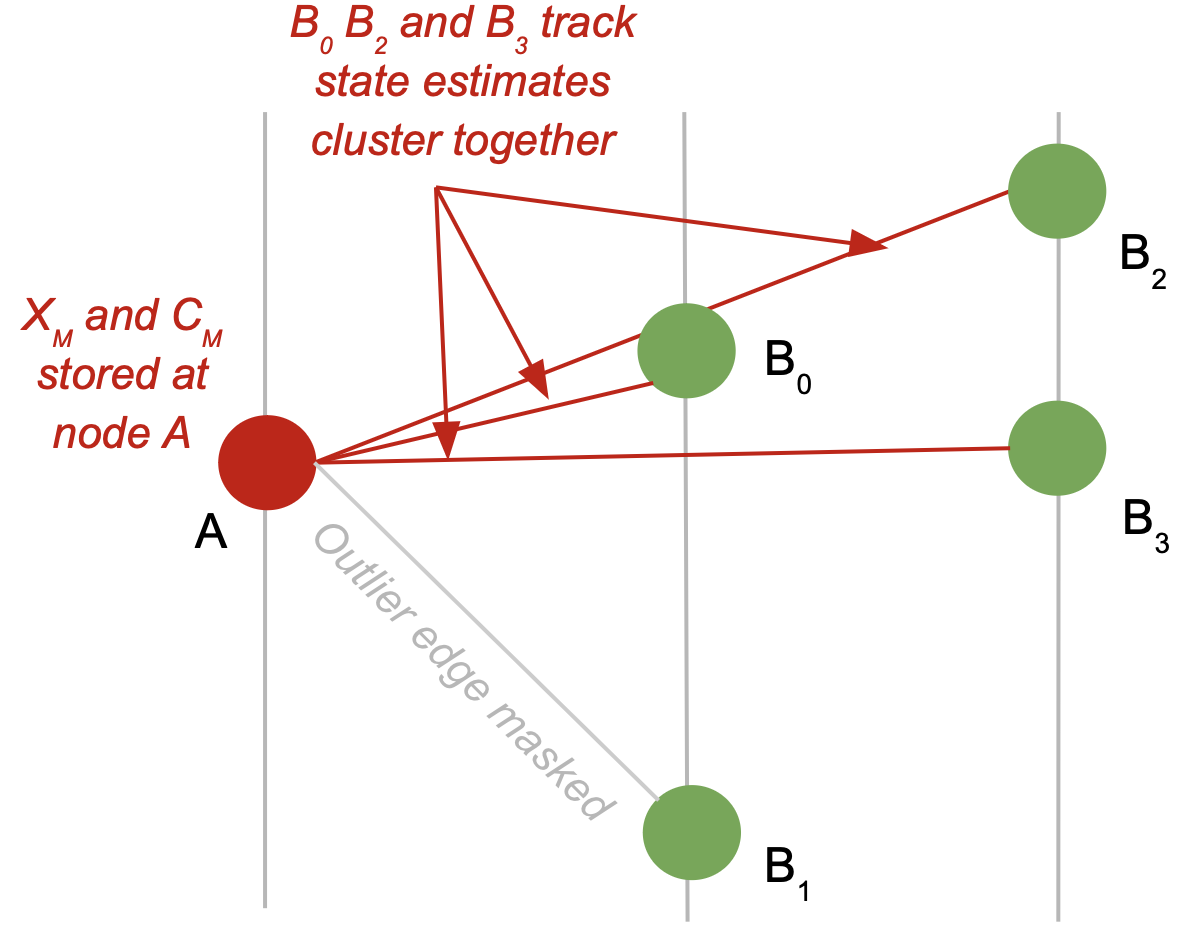
\includegraphics[width=0.57\linewidth]{images/5-gnn-algorithm/GMR-2.png}%
        \label{fig:GMR-2}%
        }%
    \caption{Illustration of GMR via clustering applied to graph networks. a) shows node $A$ and its local neighbourhood $B_j$ with bidirectional edge connections. b) shows the expected result of GMR applied to node $A$, where a merged track state $X_M$ is formed from states $X_{AB_0}$, $X_{AB_2}$, $X_{AB_3}$ clustered together and the corresponding merged state covariance $C_M$ formed from $C_{AB_0}$, $C_{AB_2}$, $C_{AB_3}$. An outlier connection has been identified, where the incoming $B_1 - A$ edge has been deactivated (dotted line) as any incoming state information from neighbour $B_1$ is deemed incompatible at node $A$.}
    \label{fig:GMR-example}
\end{figure}

The k-means clustering is implemented using the general case of $k=1$, to model the Gaussian mixture at each node as a single track with outlier connections. For the case where a node is located in close proximity to an intersection between two tracks, two or more clusters can be expected. In such a case, the mixture reduction process is declared impossible. This part of the network remains dormant until competing edges are deactivated and the mixture becomes more unimodal. 


\subsection{The Kullback-Leibler Divergence}
In order to establish whether clustering can occur for a given node, a distance measure is needed to serve as a threshold. The Kullback-Leibler (KL) divergence, $d_{KL}$, is a measure of the statistical distance between two Gaussian probability distributions \cite{KL, FRUHWIRTH19971}, and is used in the k-means algorithm to determine if track states can be grouped into a cluster. The $d_{KL}$ between track state estimates $X_{ij}$ and $X_{ik}$ is given by Eq \eqref{eqn:kullback-leibler}.

\begin{equation}
    d_{KL} = tr[(C_{ij} - C_{ik})(G_{ij} - G_{ik})] + (X_{ij} - X_{ik})^{T}(G_{ij} + G_{ik})(X_{ij} - X_{ik})
    \label{eqn:kullback-leibler}
\end{equation}

The optimal $d_{KL}$ threshold will differ for each node depending on its local neighbourhood. For example, consider a node with a high empirical variance of edge orientation in its neighbour connections, $\sigma_{e}$. The corresponding $d_{KL}$ threshold will be larger in comparison to a node with a small $\sigma_{e}$, where neighbour connections are more closely orientated. To determine the optimal $d_{KL}$ threshold between pairwise $X_{ij}$ for a given node, a SVM classifier was trained against truth information using a MC simulation. Pairwise $d_{KL}$ and $\sigma_{e}$ are used as input features. See Section \ref{chapter-6-kl-threshold} for details on the implementation of the SVM classifier.





\section{Information Aggregation}

\subsection{Message Passing}
The message passing mechanism of graph networks is leveraged in order to improve the precision of track state parameters on a local and global scale. During the previous stage (Section \ref{section-GMR}), reduced Gaussian mixtures were formed for nodes where clustering was successful. For a given node $i$, $X^M$ and $C^M$ are propagated to all neighbours $j$ which have an active $i \rightarrow j$ connection. If clustering was unsuccessful for a particular node, this part of the network remains dormant until a merged state is received via message passing during later stages of the algorithm. Track state information can be propagated in both directions along active network edges. This ensures that the compatibility of received states can be validated and assessed against each node's local neighbourhood.


\subsection{Validation}
Once state information has been propagated to neighbours, the parameter estimation begins with a linear projection of the incoming track state onto the subspace of measurements. As illustrated in Figure \ref{fig:extrapolation}, for a given node $i$ each incoming $X^M$ is projected via a measurement matrix $H$, which relates the incoming track state to the measurement values. See Section \ref{gnn-application-toy-model} for implementation of matrix $H$. In order to validate if the connection between node $i$ and $j$ is compatible, the Mahalanobis distance, $\Delta \chi^{2}_{ij}$, is calculated using the residual between the projected state, $HX$, and the measurement at the neighbour node, $m$. The threshold $d_{\chi}$ is a tuned hyperparameter and represents the maximum $\Delta \chi^{2}_{ij}$ acceptable for an incoming track state. If $\Delta \chi^{2}_{ij} < d_{\chi}$, the connection is deemed compatible and the state can be extrapolated via a KF. If $\Delta \chi^{2}_{ij} > d_{\chi}$ then the connection is deemed incompatible and the corresponding edge is deactivated.

\begin{figure}[htbp]
        \centering
        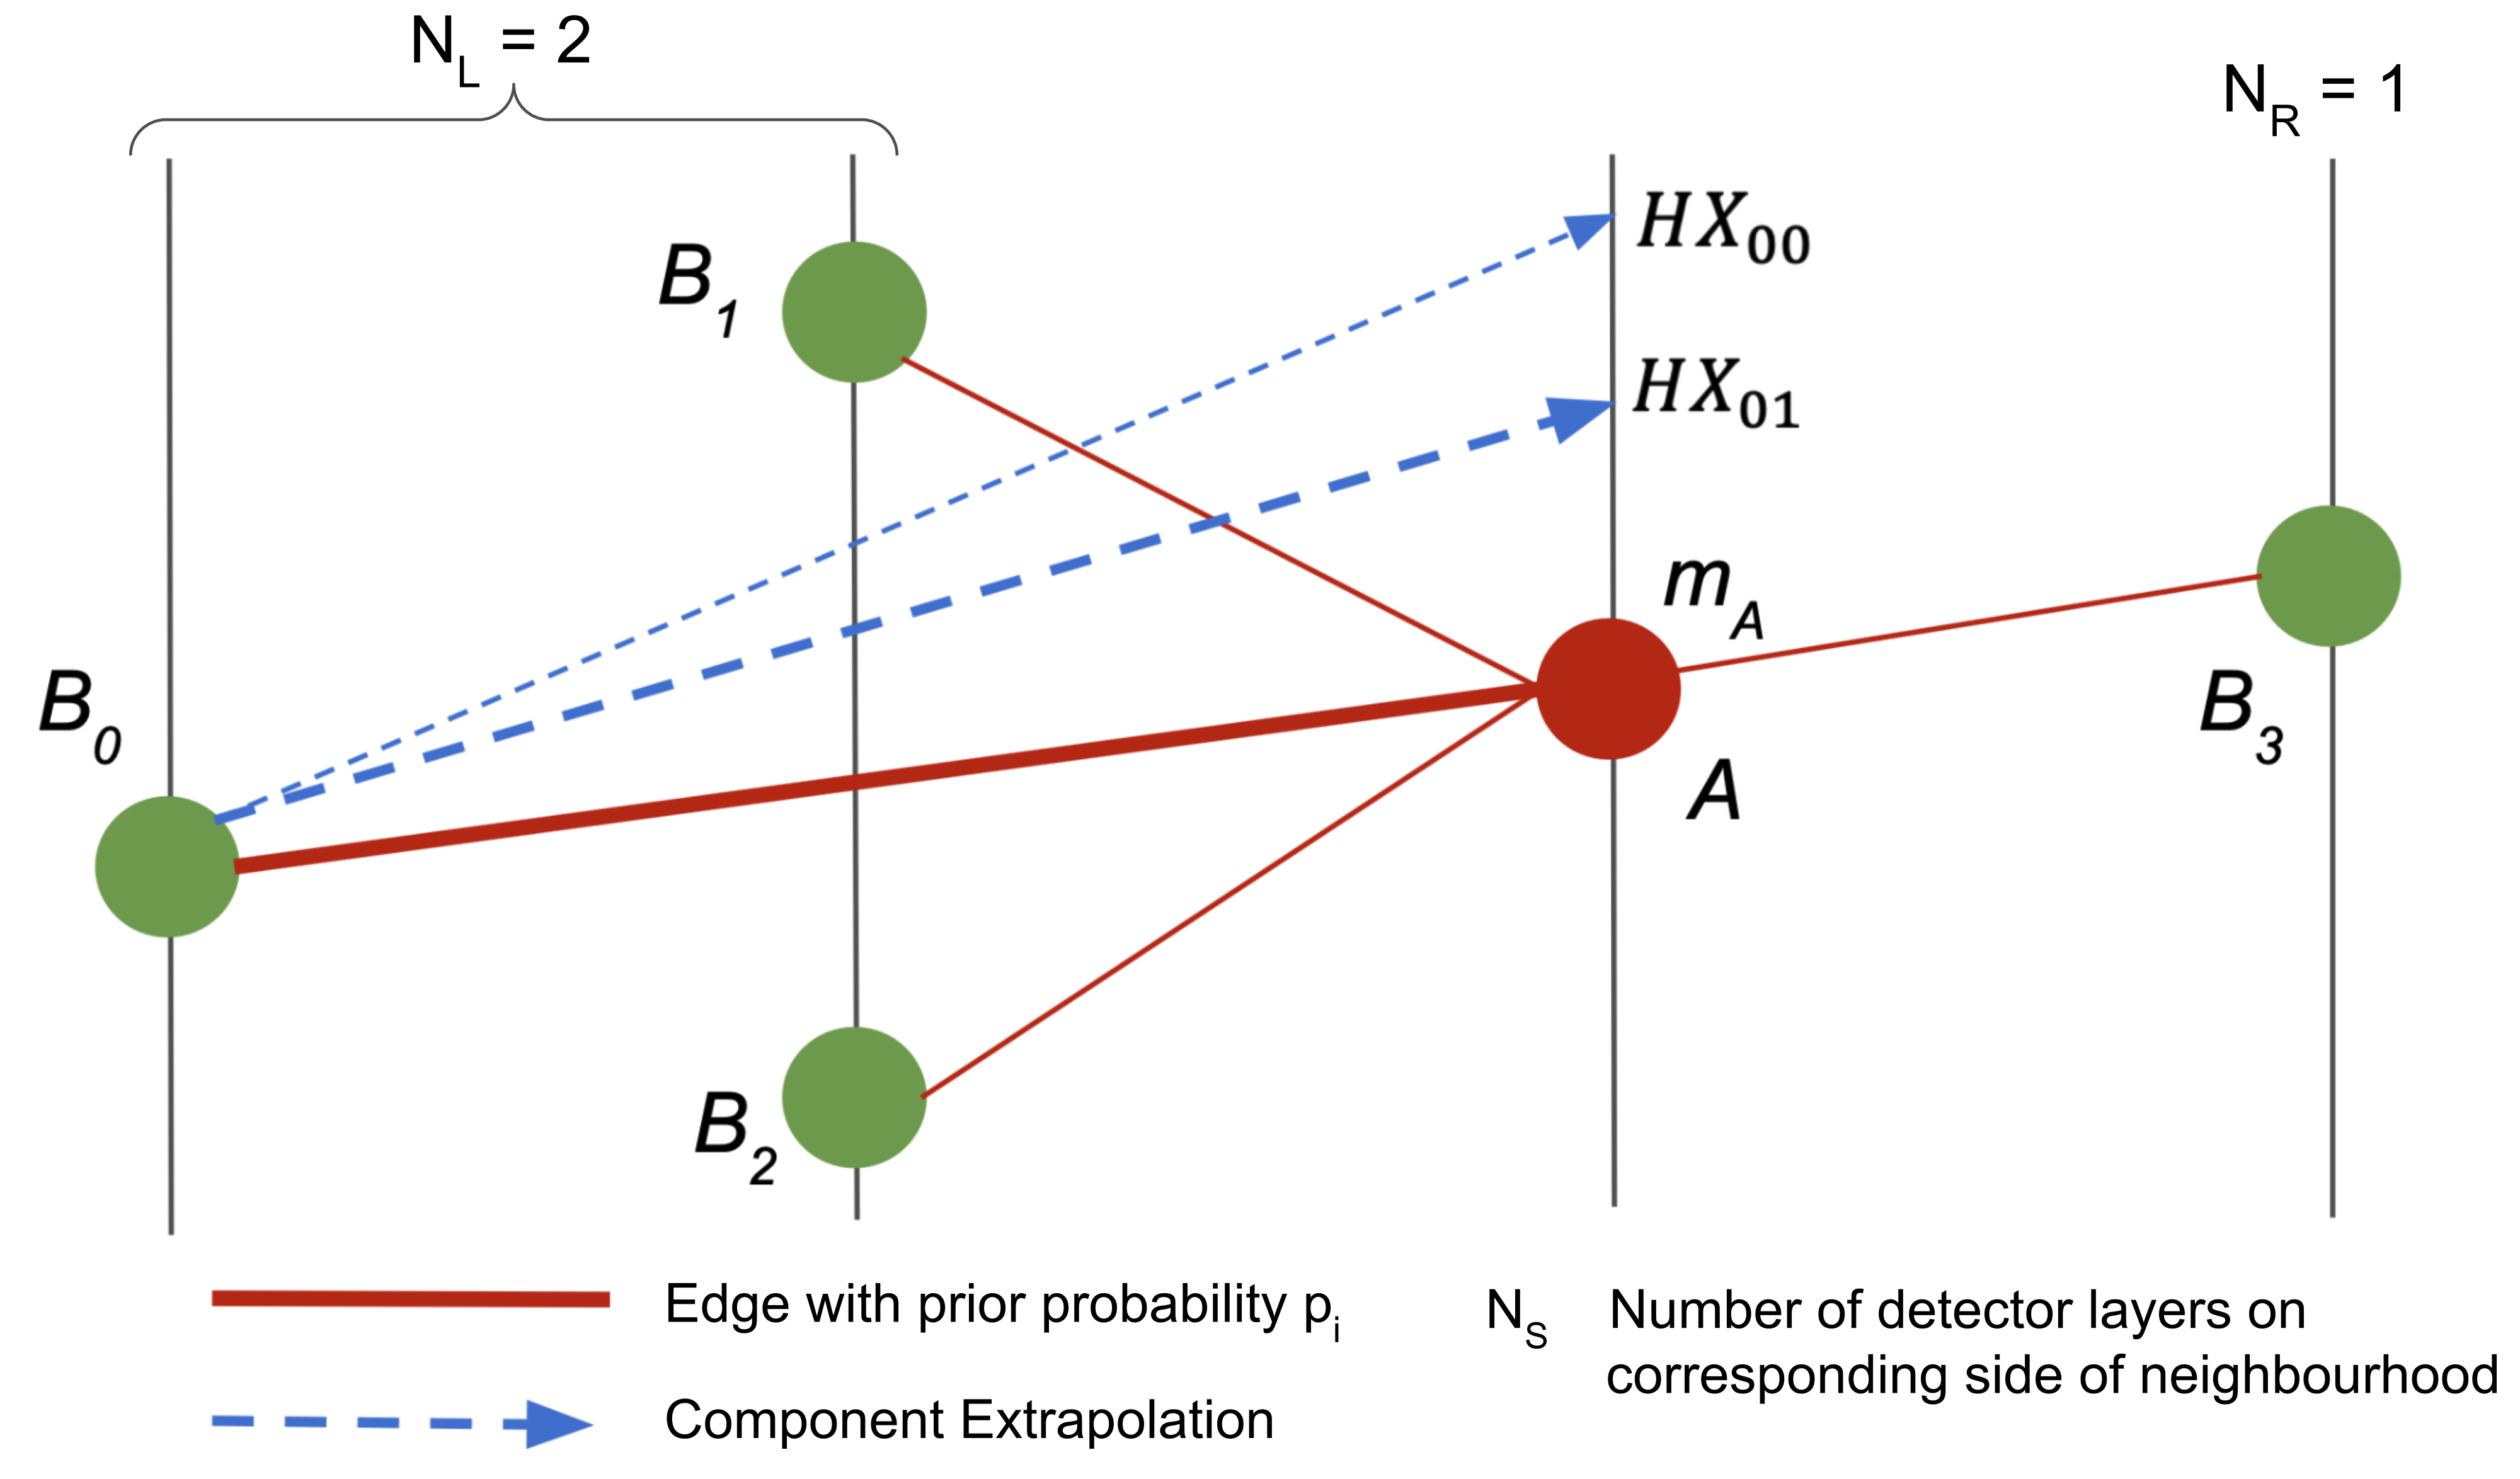
\includegraphics[width=0.87\textwidth]{images/5-gnn-algorithm/gnn-extrapolation.png}
        \caption{Illustration of track state estimates $X_{00}$ and $X_{01}$ being projected from node $B_0$ to node $A$ via a measurement matrix $H$ into the subspace of measurements. $m_A$ is the measurement at node $A$. The corresponding residual between $m_A$ and the projected incoming state from $B_0$ is used to compute the Mahalanobis distance $\Delta \chi^{2}$ to determine if the incoming state is compatible with $m_A$. $N_L$ indicates the number of detector layers on the left side of node $A$'s local neighbourhood, and $N_R$ indicates the number of detector layers on the right side.}
        \label{fig:extrapolation}%
\end{figure}


\subsection{KF Update and Extrapolation}
\label{chapter-5-kf-extrapolation}

For compatible incoming states where $\Delta \chi^{2}_{ij} < d_{\chi}$, the KF update is applied in order to compute the extrapolated track state estimate $\tilde{X}_{ij}$ and the corresponding extrapolated covariance matrix $\widetilde{C}_{ij}$. The KF is implemented via the Python library \texttt{Filterpy} \cite{filterpy}. $\tilde{X}_{ij}$ and $\widetilde{C}_{ij}$ are given by Eqs. \eqref{eqn:extrapolation},

\begin{equation}
\tilde{X}_{ij} = F_{ij} X_{ij}^{M}, \qquad \tilde{C}_{ij} = F_{ij} \biggl( \sum C_{ij}^{M} + Q \biggl) F^{T}_{ij}
\label{eqn:extrapolation}
\end{equation}

where $F_{ij}$ is the state transition Jacobian from node $i$ to node $j$, and $Q$ is the process noise matrix. See Section \ref{gnn-application-toy-model} for implementation of the KF update, including the transition Jacobian $F$ and process noise $Q$. 






\section{Updating Network State}
\label{gnn-updating-network-state}

As the network evolves and specific connections are deactivated, the local track parameter estimates change at each node. Therefore, the corresponding edge weights $w_{ij}$ should reflect this for the strength of each connection, and hence $w_{ij}$ are updated. For the connection between nodes $i$ and $j$, the updated edge weights $\widetilde{w}_{ij}$ are computed using the normalised Gaussian measurement likelihood given by Eq \eqref{eqn:likelihood} stated, where $S_{ij}$ is the joint measurement covariance matrix.

\begin{equation}
\beta_{ij} = (2 \pi \lvert S_{ij} \rvert )^{-1/2}  e^{-\Delta \chi^{2}_{ij} / 2}
\label{eqn:likelihood}
\end{equation}


The updated edge weights $\widetilde{w}_{ij}$ are given by Eq \eqref{eqn:weights}. The denominator $\sum_{k}w_{ik}\beta_{ik}$ is the summation of the product of weights and likelihoods in the neighbourhood of a given node $i$. $\widetilde{w}_{ij}$ are also divided by the number of detector layers on either side of its neighbourhood, $N_S$, in order to account for the probability that a track passing through node $i$ was detected at layer $L$. For a given node, if $\widetilde{w}_{ij} < 0.1$, the corresponding edge connection is automatically deactivated as the likelihood of compatibility of this incoming track state is extremely low. This forms part of the mechanism for edge activation and deactivation.

\begin{equation}
\widetilde{w}_{ij} = \frac{1}{N_S} \frac{w_{ij}\beta_{ij} p_{ij}}{\sum_{k}w_{ik}\beta_{ik}}
\label{eqn:weights}
\end{equation}

$g_i(X)$ at each node is then composed of updated components, given by Eq \eqref{eqn:updated-gaussian-mixture}.

\begin{equation}
g_i(X) = \sum_{j} \widetilde{w}_{ij}\phi_{ij}(X, \widetilde{X}_{ij}, \widetilde{C}_{ij})
\label{eqn:updated-gaussian-mixture}
\end{equation}

Following this update, the algorithm iterations repeat. A further GMR would follow, clustering on $\widetilde{X}_{ij}$. This allows further ambiguities to be resolved and the precision of track state parameters to be increased at each additional stage.






\section{Graph Splitting and Track Extraction}
\label{gnn-track-extration}

The GNN-based framework is designed such that it is possible to iteratively discover track candidates after each stage. As shown in Figure \ref{fig:flowchart}, a track extraction algorithm is executed after the GMR and Information Aggregation stages.

Initially, the graph network must be split into smaller components, taking into account only edges which remain active. A CCA is applied to the network by using the NetworkX built-in function \texttt{weakly\_connected\_components}. This ensures that smaller, more manageable subgraphs can be separated from the main network.

The criteria that a subgraph must possess in order to be considered for track extraction is as follows. Subgraphs must contain a minimum number of four nodes within the volume of interest. There must exist only one node per detector layer, such that there are no are intersecting tracks or holes within the track candidate. 

If the above criteria are met, a KF is then applied in order to perform a track fit. As opposed to applying the KF on one track segment between two nodes, similar to the method used in Section \ref{chapter-5-kf-extrapolation} for state extrapolation, the KF for track fitting must consider the whole chain of track segments. Here, the filter iteratively predicts and updates track state parameters as it receives $X_{ij}$ and $C_{ij}$ from each subsequent node in the subgraph.

In order to assess the quality of the track fit the p-value is computed from the $\chi^2$ statistic. The p-value obtained must be greater than 0.01. Subgraphs that fulfill all conditions are defined as good track candidates and are extracted from the network, such that their corresponding nodes and edges are removed. Subgraphs that do not meet the above criteria for track extraction, remain in the graph network for further processing.





\section{Application on a Simple MC Model}
\label{gnn-application-toy-model}

A linear 2-dimensional model was used to simulate seven truth tracks in the $x$-$y$ plane, each with ten hits as shown in Figure \ref{fig:ground-truth}. Random Gaussian noise was added to the $y$-coordinate in order to simulate measurement error. The graph network was formed using a many-to-one mapping of hits-to-nodes, where hits in close proximity within each layer were merged into one node. The threshold for close proximity was determined by considering the distance distribution between hits located in the same layer. In order to build edge connections and reduce all possible combinatorics between node pairs, an edge-predictor method was devised. The predictor uses a simple calculation whereby the track inclination of neighbour nodes is calculated. If the inclination of a neighbour node spanning up to two layers apart is within a particular range, this edge is deemed compatible and a connection is established. 

The node degree (the number of edges associated to each node) and $\sigma_e^2$ provide an indication of neighbourhood complexity. For example, nodes which have a high multiplicity of connections and regions of high node density, indicate areas with significant outliers to resolve. Nodes which have a low degree indicate areas where there are fewer ambiguities to resolve. This is illustrated by Figure \ref{fig:heat-map} showing a heat map labelled by node degree. High degree nodes are referred to as ``hot'' (white-yellow) and low degree nodes are referred to as ``cold'' (orange-red).

The network is initialised with track state estimates $X_{ij}$ given by Eq \eqref{eqn:track-state-estimate} and MC truth particle at each node. Each connection is modelled as a straight line, where $X_{ij}$ comprises of the $y$-measurement at node $i$, given by $m_i$, and the track inclination to its neighbour node $j$, given by $\tau_{ij} = (m_i - m_j) / (x_i - x_j)$. 

\begin{equation}
X_{ij} = \begin{bmatrix} m_i \\ \tau_{ij} \end{bmatrix}
\label{eqn:track-state-estimate}
\end{equation}


The joint measurement covariance matrix, $S$ is stated in Eq. \eqref{eqn:track-state-estimate-2}, where $\sigma_0^{2}$ is the error due to the measurement in the $x$-$y$ plane and is initialised to 100$\mu m$. Negligible error is assumed in the $x$ measurement due to the low thickness of Pixel sensors. Matrix $G$ relates the measurements to the state vector $X_{ij}$ using a linear extrapolation, where $dx = x_i - x_j$. The state covariance $C_{ij}$ is derived using the standard linear algebra approach, where $C_{ij} = GSG^T$. 

\begin{equation}
S = \begin{bmatrix} \sigma_0^{2} & 0 \\ 0 & \sigma_0^{2} \end{bmatrix}  \quad G = \begin{bmatrix} 1 & 0 \\ dx^{-1} & -dx^{-1}  \end{bmatrix}
\label{eqn:track-state-estimate-2}
\end{equation}


During GMR via clusterisation, $X^{M}$ and $C^{M}$ were computed using Eq \eqref{eqn:inverse-variance-weighting}. During the Information Aggregation stage, $X^M$ were projected into the subspace of measurements using the measurement vector $H = [1 \quad 0]$. The residual, $r_{ij}$, was then calculated between the projection, $HX^M$, and the measurement at each node using $r_{ij} = m_i - HX_{ij}^M$. The covariance of $r_{ij}$ is given by Eq. \eqref{eqn:covariance-of-residual}

\begin{equation}
\hat{C}_{ij} = H \widetilde{C}_{ij} H^{T} + \sigma_{0}^{2}
\label{eqn:covariance-of-residual}
\end{equation}

where the process noise $Q$ in computing $\widetilde{C}_{ij}$ is defined as the zero matrix for simplicity. The corresponding Mahalanobis distance is given by Eq \eqref{eqn:mahalanobis-distance}.

\begin{equation}
\Delta \chi_{ij}^{2} = r_{ij}^{T} \hat{C}_{ij}^{-1} r_{ij}
\label{eqn:mahalanobis-distance}
\end{equation}

If $\Delta \chi_{ij}^{2} < 1$, then $X^M$ is extrapolated to its neighbour node. The extrapolated state, $\widetilde{X}_{ij}$, is calculated using \eqref{eqn:extrapolation} defined as the linear extrapolation from node $j$ to node $i$, given by $m_i = m_j + \tau_j dx$ and $\tau_i = \tau_j$. Therefore, the derived Jacobian is given by Eq \eqref{eqn:mc-model-F}.

\begin{equation}
F = \begin{bmatrix} 1 & dx \\ 0 & 1 \end{bmatrix}
\label{eqn:mc-model-F}
\end{equation}



\begin{center}
\begin{figure}[htbp]%
    \centering
    \subfloat[\centering Simulation of seven truth tracks]{{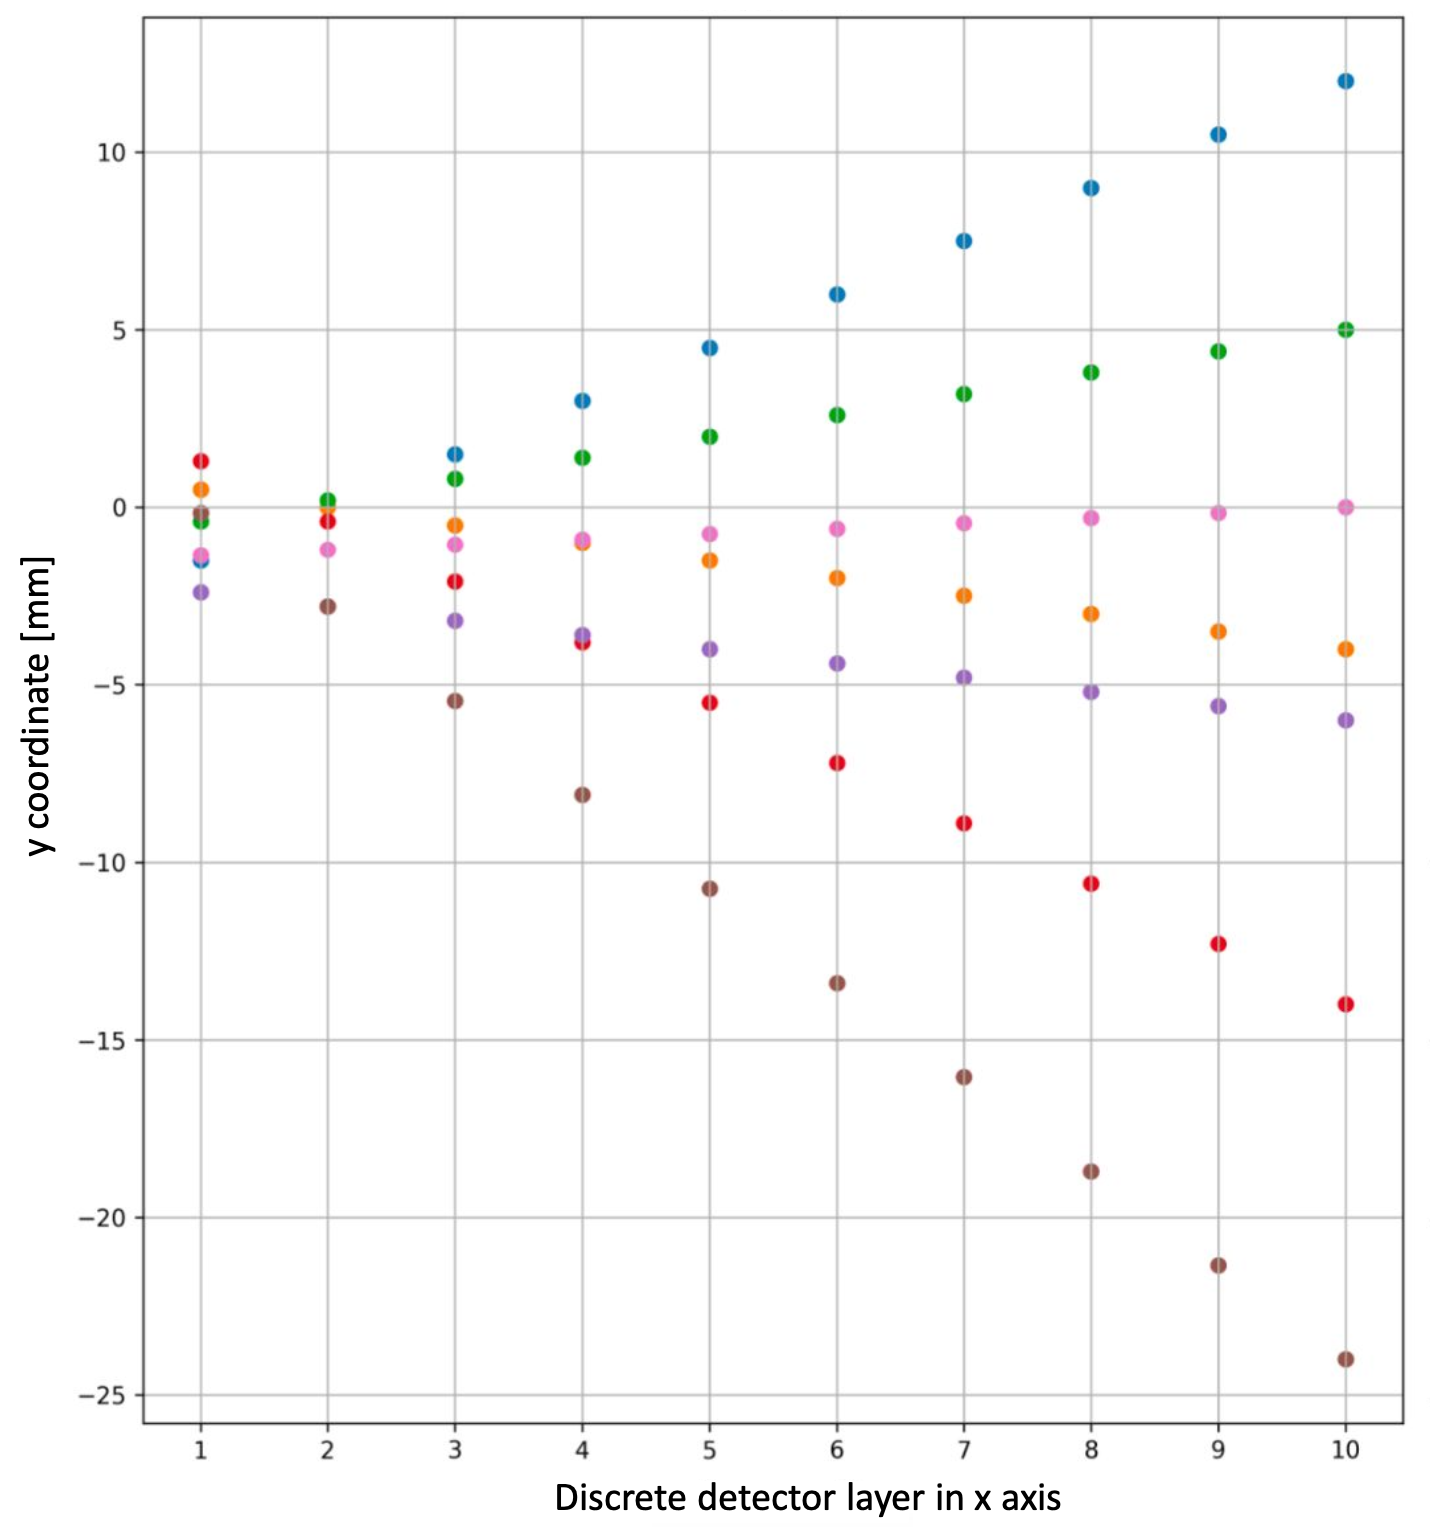
\includegraphics[width=8cm]{images/5-gnn-algorithm/ground-truth.png} } \label{fig:ground-truth}}%
    \hfill
    %\qquad
    \subfloat[\centering Graph network plotted as a node-degree heat map]{{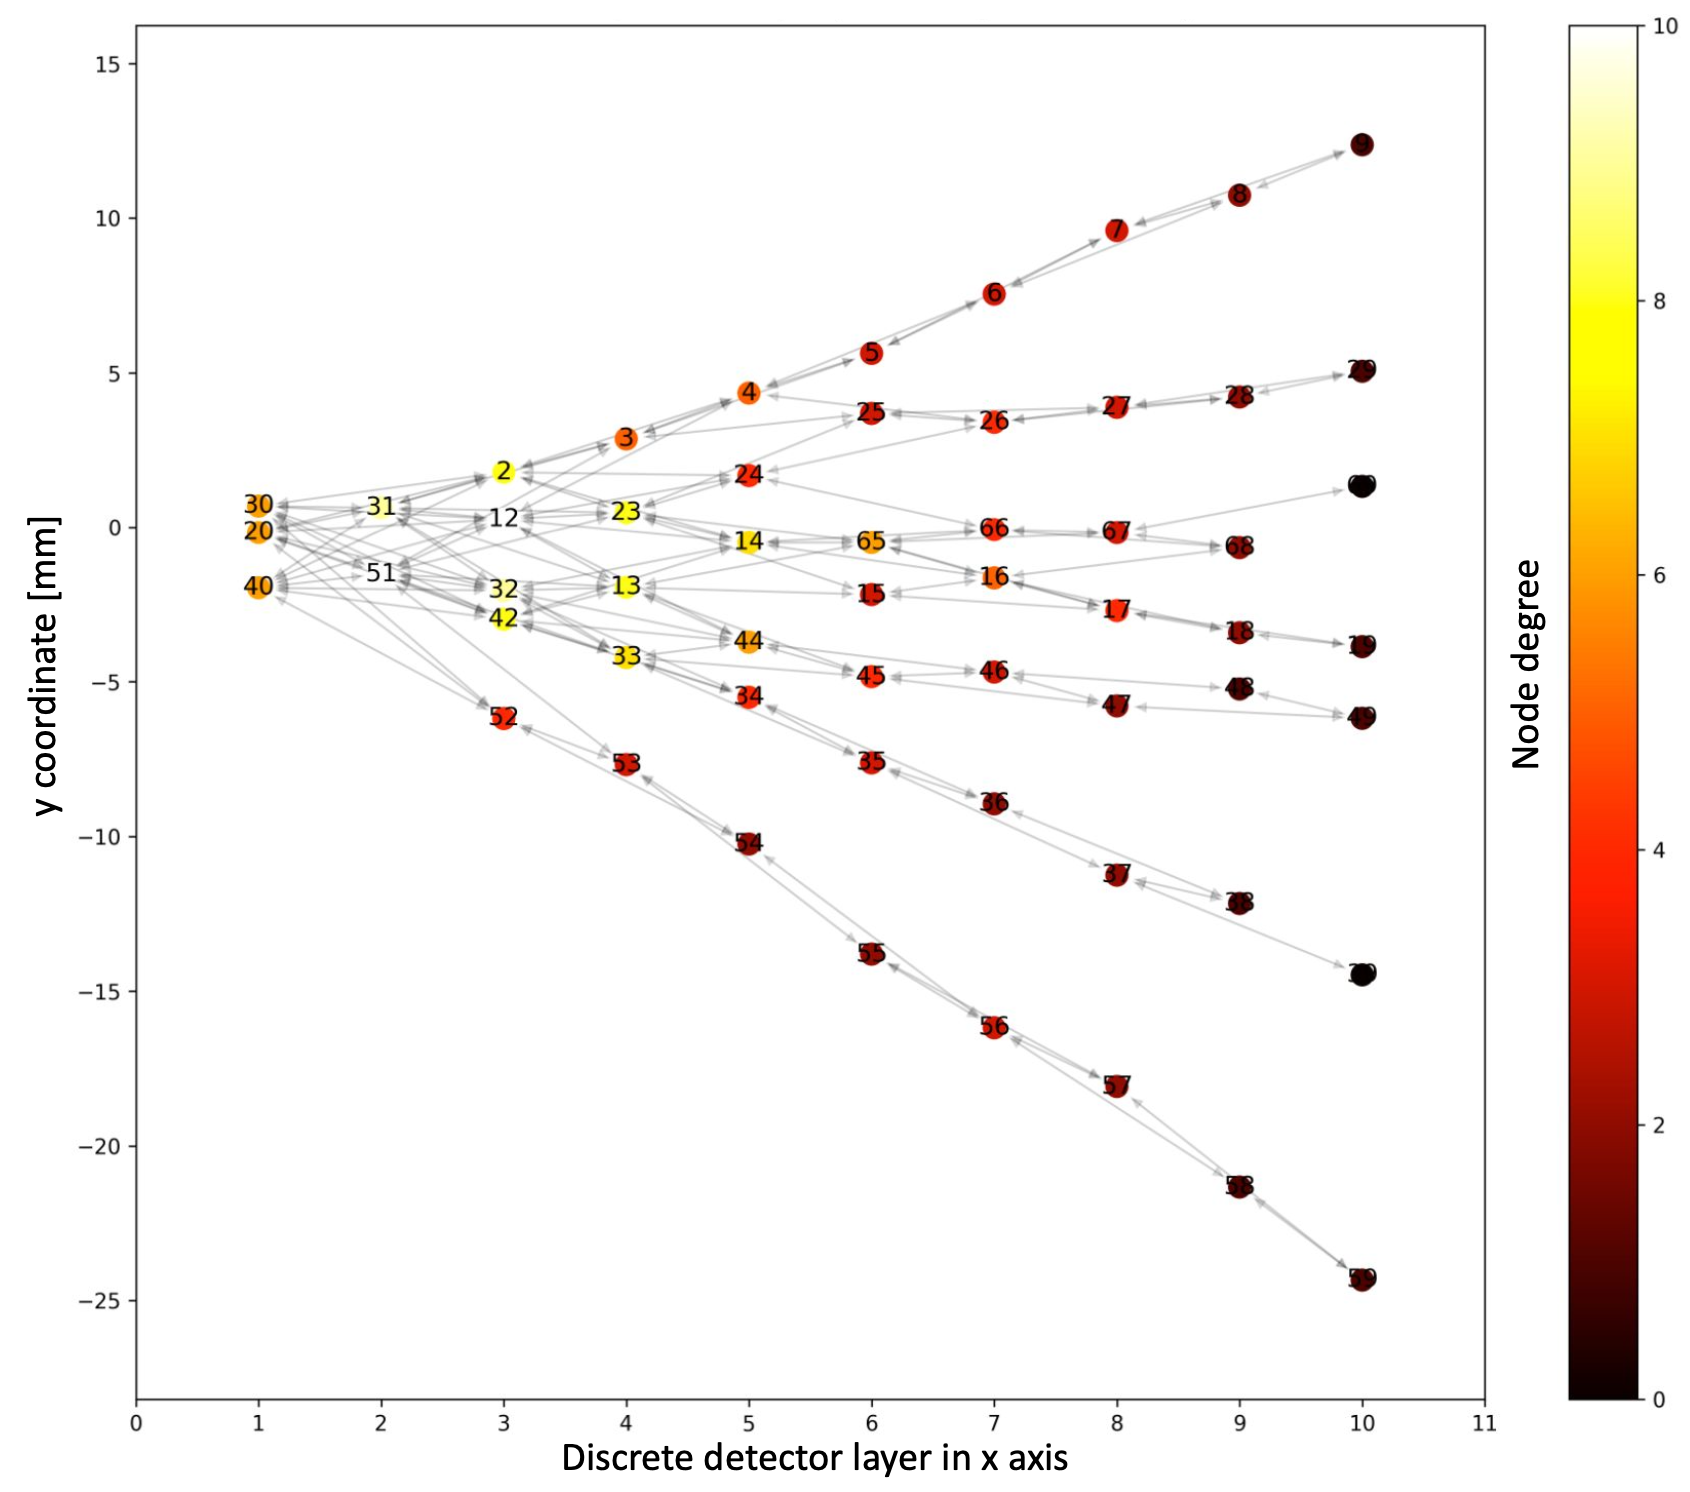
\includegraphics[width=11cm]{images/5-gnn-algorithm/heatmap-network.png} } \label{fig:heat-map}}%
    \caption{a) Simple 2-dimensional simulation of seven truth tracks where each track contains ten hits; one hit per layer. Each colour represents a different track. b) Conversion of the simulated hits in a), to a graph network containing nodes and edges. Close proximity hits are merged into the same node where necessary and predicted edge connections are formed using a pair predictor. The heat map represents node degree, where ``hot'' nodes (white-yellow) contain many edge connections, whereas ``cold'' nodes (orange-red) contain fewer edge connections.}%
    \label{fig:setup}%
\end{figure}
\end{center}



Figure \ref{fig:example-application-1} shows an example of the GNN algorithm applied to the simulated network in Figure \ref{fig:heat-map}. Figure \ref{fig:mc-example-1} displays the graph network where an initial CCA has been applied. Three smaller subgraphs have been identified as shown by the separate colours. The subsequent extracted track candidates from this network are shown in Figure \ref{fig:mc-example-2}, where seven distinct tracks can be observed. Outlier edge connections have been successfully identified and no longer visible. This particular simulation shows 100\% purity of track reconstruction with respect to MC truth, as all seven truth tracks have been successfully extracted within two stages. Nodes with $\sigma_e^2 > 0.8$ are not shown here, as clustering was not possible. This indicates that the GNN algorithm behaved as expected, resolving ambiguities in cold node regions during the first and second stages.

Figure \ref{fig:example-application-2} shows another simulation of a simple track model with application of the GNN algorithm. The application of CCA yields two distinct subgraphs shown in Figure \ref{fig:mc-example-3}. The subsequent extracted track candidates are shown in Figure \ref{fig:mc-example-4}, where six distinct tracks can be observed. A precision of 65\% was achieved on identifying correct outlier connections with respect to the MC truth during stage 1. A fast convergence was achieved in extracting 6 out of 7 candidates after the first stage of the algorithm. Remaining networks were propagated to further stages, however no further track candidates were extracted. Similarly, nodes with $\sigma_e^2 > 0.8$ are not shown here, as clustering was not possible. This suggests that $\sigma_{e}$ is an important discriminating feature when clustering track state estimates. 

From the example simulations, it was observed that clustering of states was not always possible in all hot node regions. As a result, the pattern recognition process was automatically initiated in regions where outlier connections were easily identifiable, i.e. cold nodes regions. This indicates that an intrinsic characteristic of the GNN algorithm is that neighbourhood complexity is inherently known by the network. 

\begin{center}
\begin{figure}[htbp!]%
    \centering
    \subfloat[\centering Simulated graph network. CCA used to separate the main network into three smaller subgraphs, indicated by each colour]{{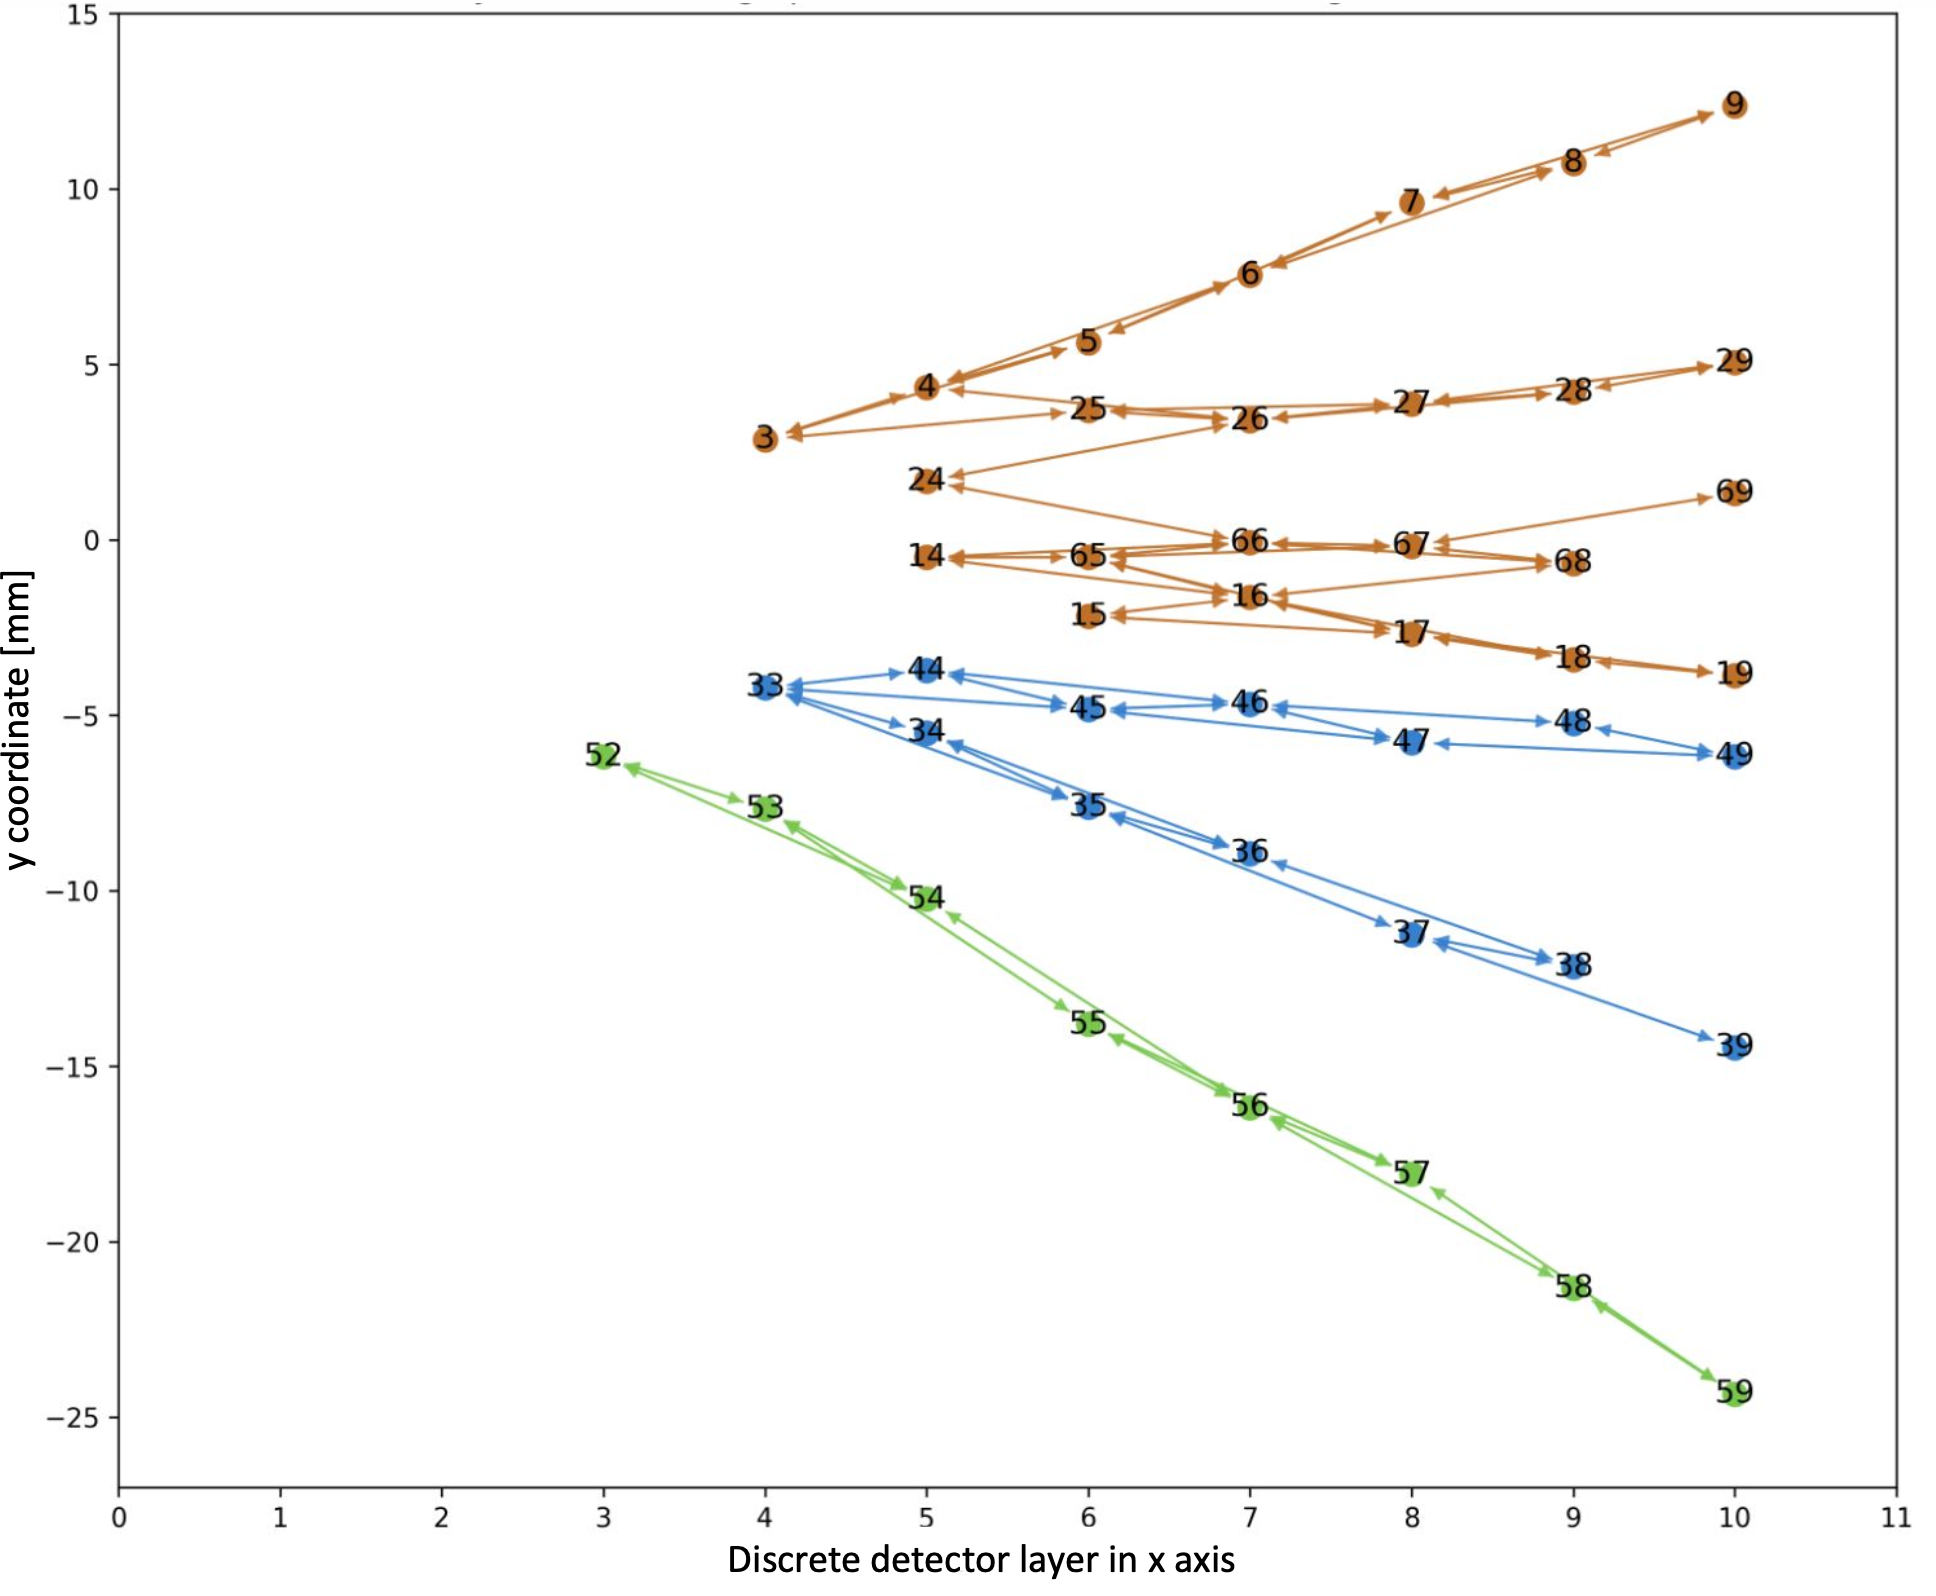
\includegraphics[width=10.5cm]{images/5-gnn-algorithm/mc-example-1.png} } \label{fig:mc-example-1}}%
    \hfill
    %\qquad
    \subfloat[\centering Extracted track candidates at each stage of the GNN algorithm]{{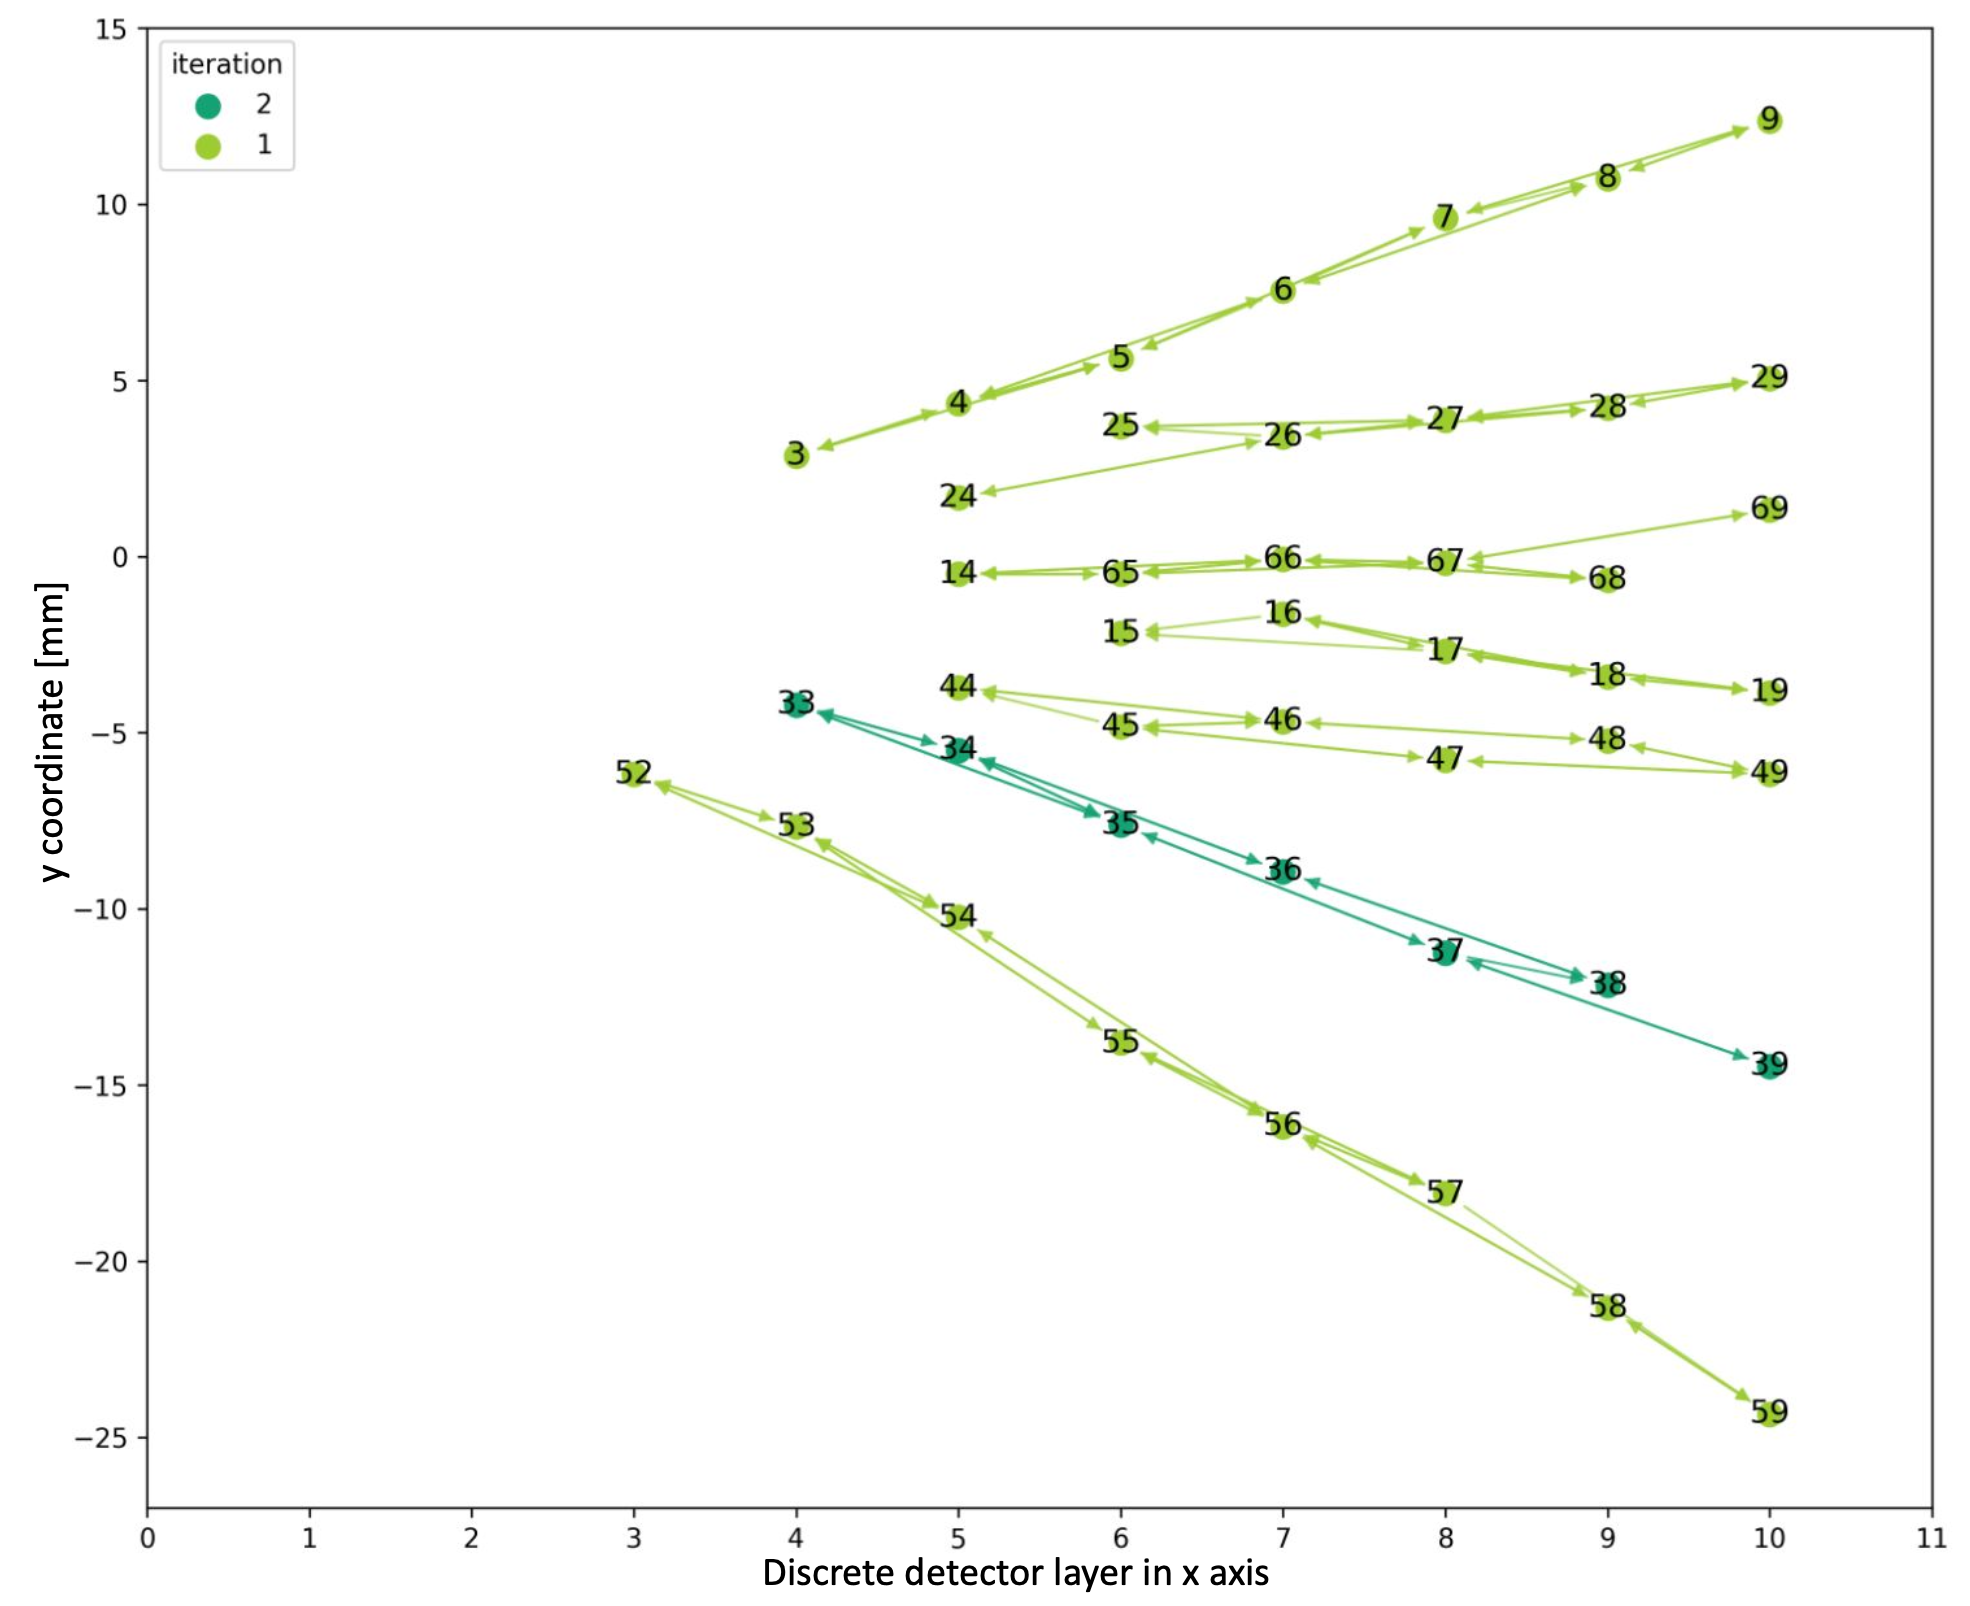
\includegraphics[width=11cm]{images/5-gnn-algorithm/mc-example-2.png} } \label{fig:mc-example-2}}%
    \caption{Results of the GNN-based algorithm applied to a simple MC simulation a) shows the simulated graph network where nodes $\sigma_e^2 > 0.8$ are removed and a CCA is applied to split the graph network into three smaller subgraphs, where each colour indicates a different subgraph. b) Shows the extracted track candidates after the applied GMR and Information Aggregation stages, where seven separate tracks can be seen.}%
    \label{fig:example-application-1}%
\end{figure}
\end{center}

\begin{center}
\begin{figure}[htbp!]%
    \centering
    \subfloat[\centering Simulated graph network post CCA]{{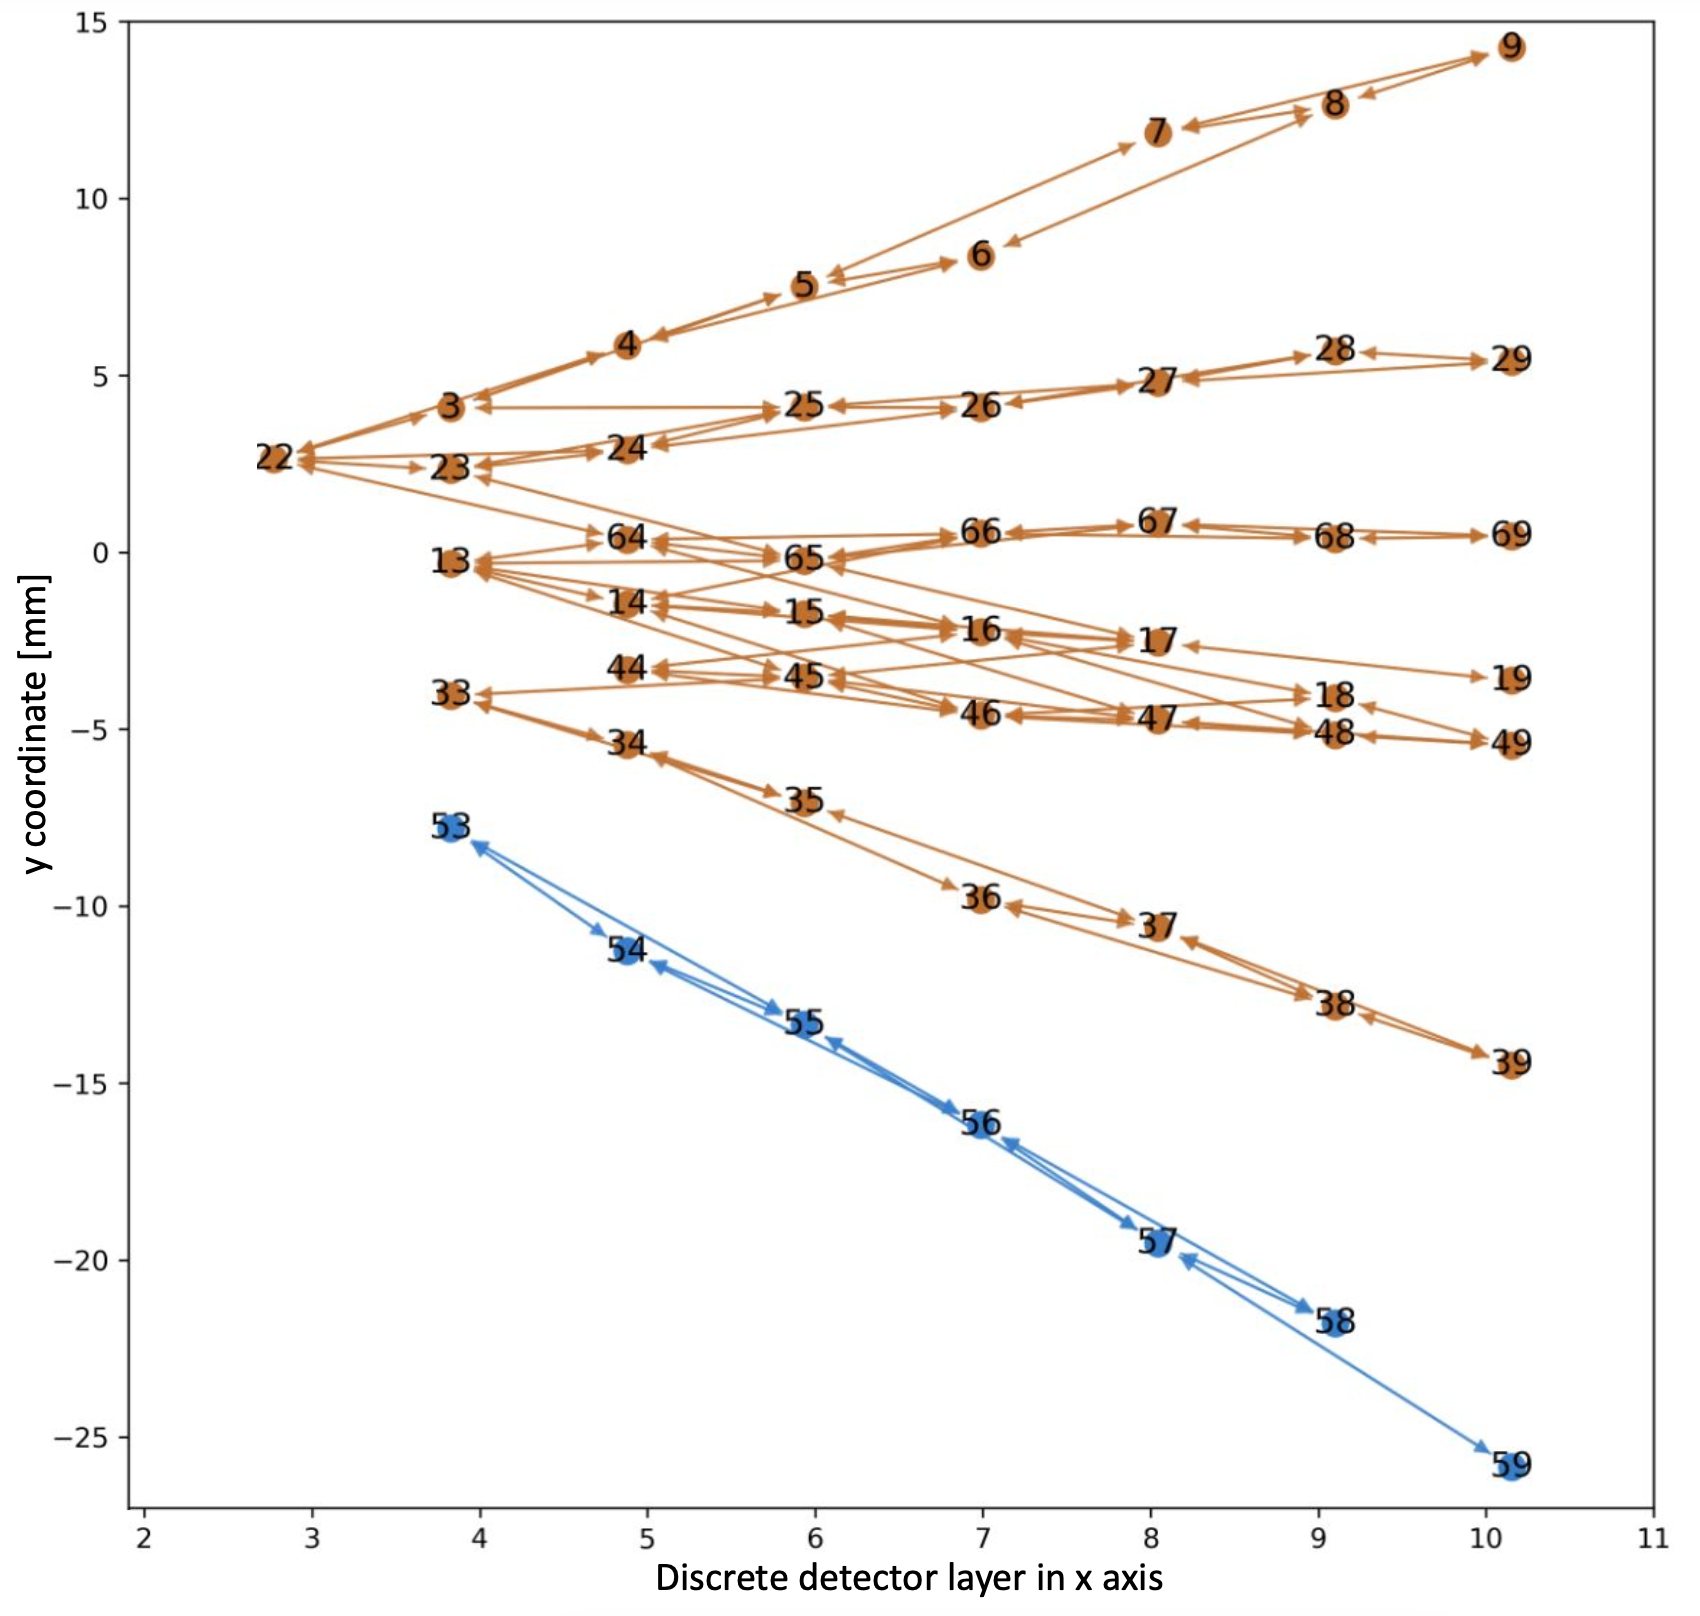
\includegraphics[width=9.2cm]{images/5-gnn-algorithm/mc-example-3.png} } \label{fig:mc-example-3}}%
    \hfill
    %\qquad
    \subfloat[\centering Extracted track candidates after stage 1]{{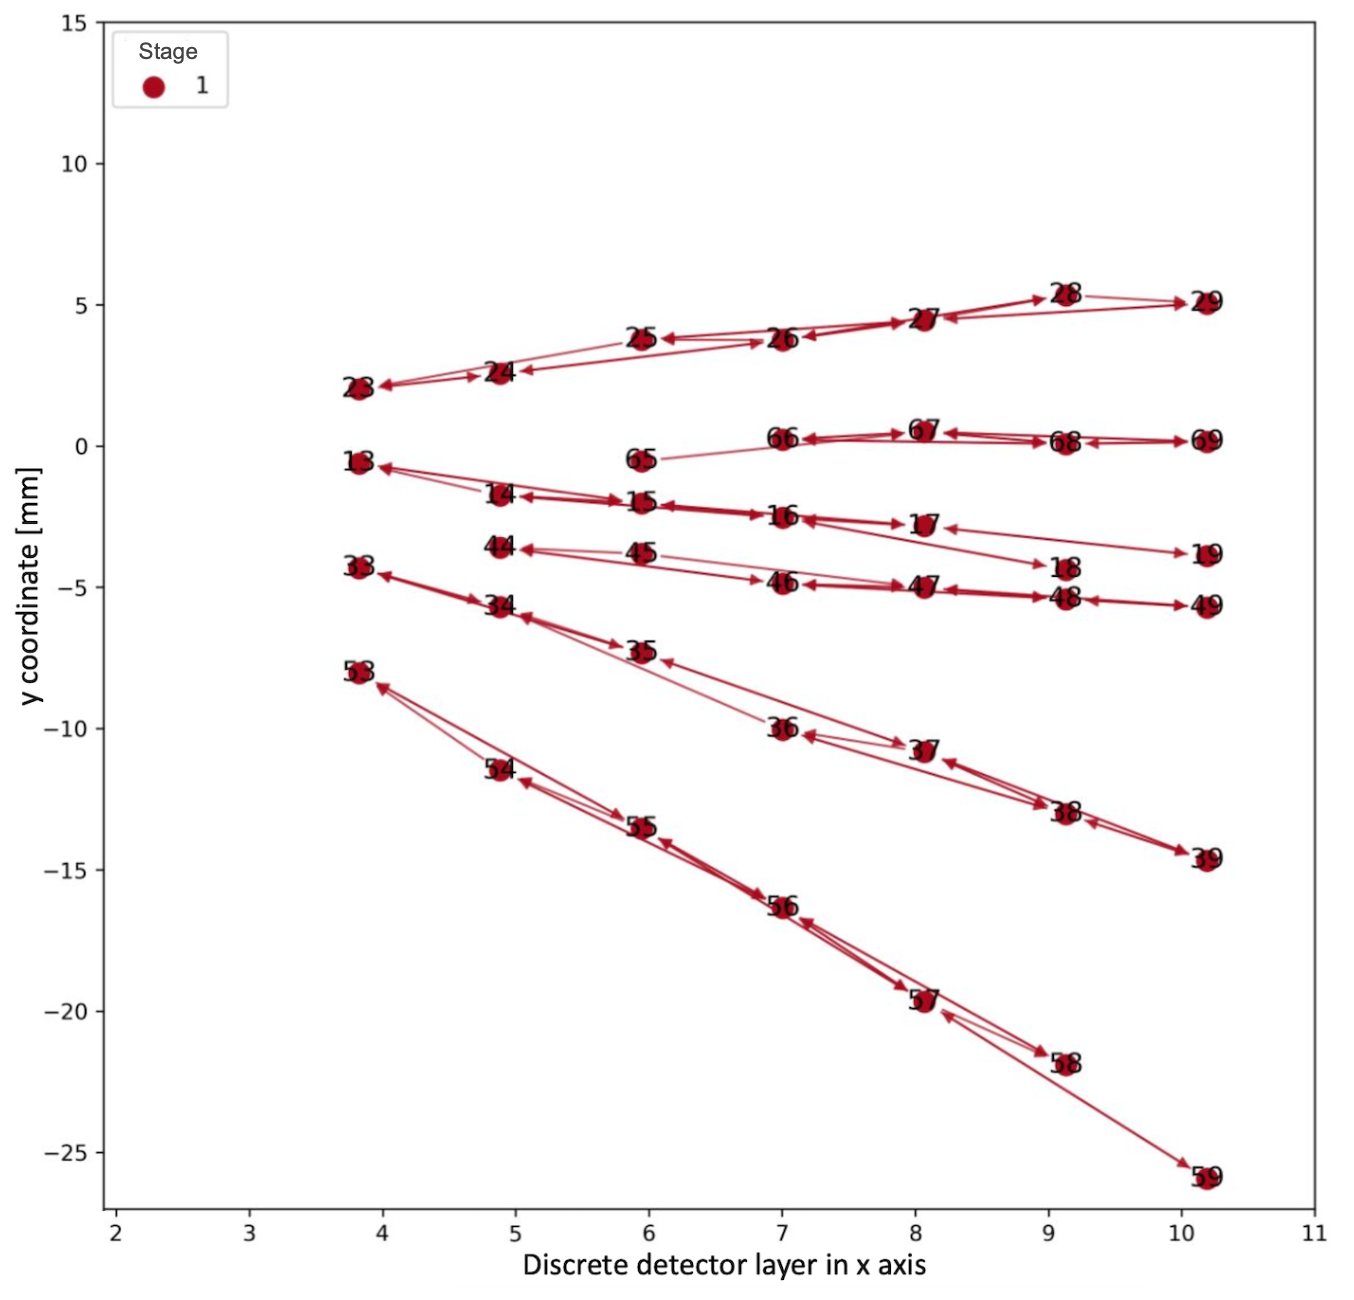
\includegraphics[width=9.6cm]{images/5-gnn-algorithm/mc-example-5.png} } \label{fig:mc-example-4}}%
    \caption{Results of the GNN-based algorithm applied to a simple MC simulation a) shows the simulated graph network where nodes $\sigma_e^2 > 0.8$ are removed and a CCA is applied to split the graph network into two smaller subgraphs, where each colour indicates a different subgraph. b) shows the resulting network post GMR. The faded grey connections represents deactivated outlier edges. c) Shows six extracted track candidates after the applied GMR.}%
    \label{fig:example-application-2}%
\end{figure}
\end{center}

\section{Conclusions}

The proposed GNN algorithm is successful in iteratively identifying outlier edge connections and extracting track candidates for simple simulated particle collision events. GMR via clustering of state vectors proves to be a successful first step towards resolving incompatible connections in the network. The KF works well for both the extrapolation of state vectors to neighbour nodes in order to learn neighbourhood information and improve the precision in track state parameters, as well as for track fitting and extraction. The GNN algorithm automatically initiates the pattern recognition process in regions where outlier connections are easily identifiable. The network starts with low density regions and gradually progresses towards high density areas. This indicates that the GNN algorithm shows great promise for extraction of track candidates in more complex cases and realistic detector setups.